\begin{figure}[htbp]

  \centering
  %\begin{tabular}[t]{c}
  \usetikzlibrary{positioning,matrix, arrows.meta}
\usetikzlibrary{shapes,arrows}

\tikzstyle{block} = [draw, rectangle, 
    minimum height=3em, minimum width=6em,fill=blue!30]
\tikzstyle{circ} = [draw, circle, node distance=1cm,fill=red!30]
\tikzstyle{input} = [coordinate]
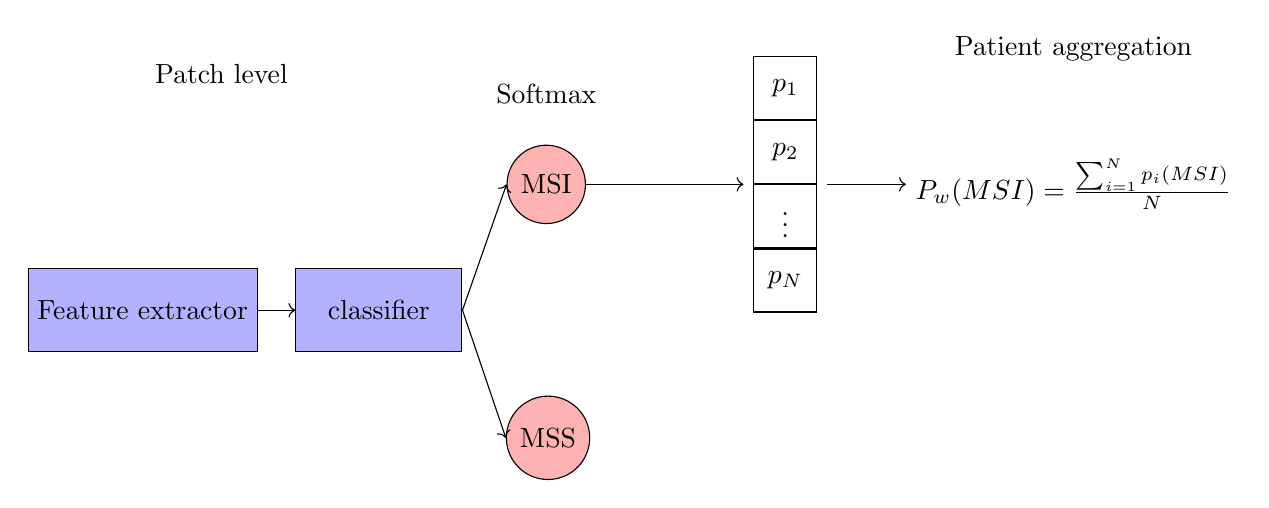
\begin{tikzpicture}
\node [input, name=input] {};
\node [block] (inception) at (0,0) {Feature extractor};
\node [block] (mlp) at (3,0) {classifier};
\node(D) at(1,3) {Patch level};
\node [circ, above right=of mlp] (msi) {MSI};
\node(C) [above=0.4cm of msi]{Softmax};
\node [circ, below right=of mlp] (mss) {MSS};
\matrix (A) [matrix of nodes, right=2cm of msi, nodes={draw, minimum size=8mm},column sep=-\pgflinewidth]
{    $p_1$\\$p_2$\\\vdots\\$p_N$\\};
\node(B)[right=of A]{
    \(P_w(MSI) = \frac{\sum_{i=1}^{N}p_i(MSI)}{N}\)};
\node(C) [above=of B]{Patient aggregation};
\draw [->] (inception.east) -- (mlp.west);
\draw [->] (mlp.east) -- (msi.west);
\draw [->] (mlp.east) -- (mss.west);
\draw [->] (msi.east) -- (A.west);
\draw[->] (A.east) -- (B.west);
\end{tikzpicture}
\\ (a)\\
  
  \usetikzlibrary{positioning,matrix, arrows.meta}
\usetikzlibrary{shapes,arrows}

\tikzstyle{block} = [draw, rectangle, 
    minimum height=3em, minimum width=6em,fill=blue!30]
\tikzstyle{circ} = [draw, circle, node distance=1cm,fill=red!30]
\tikzstyle{input} = [coordinate]
\begin{tikzpicture}
\node [input, name=input] {};
\node [block] (inception) at (0,0) {Feature extractor};
\node [block] (mlp) at (3,0) {classifier};
\node(D) at(1,3) {Patch level};
\node [circ, above right=of mlp] (msi1) {$MSI_1$};
\node(C) [above=0.4cm of msi]{Softmax};
\node [circ, below right=of mlp] (mss) {MSS};
\node [circ, right=0.4cm of mlp] (msi2) {$MSI_2$};
\matrix (A) [matrix of nodes, right=3cm of msi1, nodes={draw, minimum size=8mm},
    column sep=-\pgflinewidth]{
    $p_1$\\$p_2$\\\vdots\\$p_N$\\};
\node(B)[right=of A]{
    \(P_w(MSI) = \frac{\sum_{i=1}^{N}p_i(MSI)}{N}\)};
\node(C) [above=of B]{Patient aggregation};
\draw [->] (inception.east) -- (mlp.west);
\draw [->] (mlp.east) -- (msi1.west);
\draw [->] (mlp.east) -- (msi2.west);
\draw [->] (6.5,1) -- (8.5,1) node[midway,above]{max($MSI_1$,$MSI_2$)};
\draw [->] (mlp.east) -- (mss.west);
\draw[->] (A.east) -- (B.west);
\end{tikzpicture}
\\ (b)
  %\end{tabular}
    \caption{ Baseline model architecture. Patches are inputted to Inception-Net for feature extraction. Final 2 layers are fully connected  classifier layers. Outputs are propagated to a softmax layer for probabilities. N is number of patient patches, $P_i$ are patches MSI probabilities. $P_w$, MSI score for each patient is average over its MSI probabilities (a). Biologically-primed model architecture. As in the baseline, the softmax layer output classes probabilities in patch-level. The MSI probability is the max between $MSI_1$ and $MSI_2$ outputs. $P_w$ same as in baseline (b).}
  \label{fig:net_arch}
\end{figure}